%%%%%%%%%%%%%%%%%%%%%%%%%%%%%%%%%%%%%%%%%
% Science Communication
% 2016SoE022
% Portland State University (Fall 2016)
% Author: bmarron
% Creation date: 05 Nov 2016
%%%%%%%%%%%%%%%%%%%%%%%%%%%%%%%%%%%%%%%%


% Careful with directory name for graphics
% Note date
% Slides begin line 227


% The class {scrartcl} pro­vides the “ar­ti­cle”-like el­e­ment of the koma-script col­lec­tion.
% The doc­u­ment lay­out of the class is less ‘stri­dent’ than that of ar­ti­cle, and it of­fers 
% much more flex­i­bil­ity than ar­ti­cle via other el­e­ments of the koma-script col­lec­tion. 
% https://www.ctan.org/pkg/scrartcl?lang=en
% https://www.ctan.org/topic/class

%----------------------------------------------------------------------------------------
%	PACKAGES AND OTHER DOCUMENT CONFIGURATIONS
%----------------------------------------------------------------------------------------
\documentclass[
paper=128mm:96mm, % The same paper size as used in the beamer class
fontsize=11pt, % Font size
pagesize, % Write page size to dvi or pdf
parskip=half-, % Paragraphs separated by half a line
]{scrartcl} 

\linespread{1.12} % Increase line spacing for readability

%--------- Required packages ------------------------------------------------
\usepackage{xcolor}	 % Required for custom colors
% Define a few colors for making text stand out within the presentation
% Use these colors within the presentation by enclosing text in the commands below
\definecolor{mygreen}{RGB}{44,85,17}
\definecolor{myblue}{RGB}{34,31,217}
\definecolor{mybrown}{RGB}{194,164,113}
\definecolor{myred}{RGB}{255,66,56}
\newcommand*{\mygreen}[1]{\textcolor{mygreen}{#1}}
\newcommand*{\myblue}[1]{\textcolor{myblue}{#1}}
\newcommand*{\mybrown}[1]{\textcolor{mybrown}{#1}}
\newcommand*{\myred}[1]{\textcolor{myred}{#1}}

\usepackage[includeheadfoot,
top=3.5mm,
bottom=3.5mm,
left=5.5mm,
right=5.5mm,
headsep=6.5mm,
footskip=8.5mm
]{geometry} % Page margins settings

\usepackage[T1]{fontenc}	                    % Fonts, for correct hyphenation and T1 encoding
\usepackage{lmodern}                          % Default font: latin modern font
	%\usepackage{fourier}                       % Alternative font: utopia
	%\usepackage{charter}                       % Alternative font: low-resolution roman font
\renewcommand{\familydefault}{\sfdefault}     % Sans serif - this may need to be commented to see the alternative fonts
\usepackage{amsmath}
\usepackage{amsthm}                           % Required for theorem environments
\usepackage{bm}                               % Required for bold math symbols (used in the footer of the slides)
\usepackage{graphicx}                         % Required for including images in figures
\usepackage{booktabs}                         % Required for horizontal rules in tables
\usepackage{multicol}                         % Required for creating multiple columns in slides
\setlength{\columnsep}{0.1mm}

\usepackage{lastpage}                         % For printing the total number of pages at the bottom of each slide
\usepackage[english]{babel}                   % Document language - required for customizing section titles
\usepackage{microtype}                        % Better typography
\usepackage{tocstyle}                         % Required for customizing the table of contents
\usepackage{caption}
\captionsetup{labelformat=empty,labelsep=none}
\usepackage{mathtools}
\usepackage{subcaption}
\usepackage{nicefrac}
\usepackage{csquotes}
\usepackage{enumitem}	%spread enumeration over multiple slides
\usepackage{pdfpages}
\usepackage{tikz}  
\usepackage[absolute, overlay]{textpos}      %position textblocks (absolute) on the page
\setlength{\TPHorizModule}{\textwidth}
\setlength{\TPVertModule}{\textwidth}

\usepackage{scrpage2}                       % Slide layout configuration; Required for customization of the header and footer
\pagestyle{scrheadings}                     % Activates the pagestyle from scrpage2 for custom headers and footers
\clearscrheadfoot                           % Remove the default header and footer
\setkomafont{pageheadfoot}{
\normalfont\color{black}\sffamily
}                                            % Font settings for the header and footer

\usepackage{titlesec}                       % Required for customizing section spacing
\titlespacing{\section}{0mm}{0mm}{0mm}      % Lengths are: left, before, after
\titlespacing{\subsection}{0mm}{0mm}{-1mm}  % Lengths are: left, before, after
\titlespacing{\subsubsection}{0mm}{0mm}{-2mm} % Lengths are: left, before, after
\setcounter{secnumdepth}{0}                 % How deep sections are numbered, set to no numbering by default
                                            % change to 1 for numbering sections, 2 for numbering sections and subsections, etc

% Presentation mode (uncomment for full screen)
%\usepackage{hyperref} 
%\hypersetup{pdfpagemode=FullScreen}



%---------- Sets vertical centering of slide contents with increased space between paragraphs/lists ---------------
\makeatletter
\renewcommand*{\@textbottom}{\vskip \z@ \@plus 1fil}
\newcommand*{\@texttop}{\vskip \z@ \@plus .5fil}
\addtolength{\parskip}{\z@\@plus .25fil}
\makeatother

%----------- Remove page numbers and the dots leading to them from the outline slide ------------------------------
\makeatletter
\newtocstyle[noonewithdot]{nodotnopagenumber}{\settocfeature{pagenumberbox}{\@gobble}}
\makeatother
\usetocstyle{nodotnopagenumber}

%-------- Change the name of the table of contents -----------------------------------------------
\AtBeginDocument{\renewcaptionname{english}{\contentsname}{\Large Outline}} 


%---------- Header configuration ---------------------------------------------------------------
\ihead{
\hspace{-2mm}
\begin{tikzpicture}[remember picture,overlay]
                                            % Colored bar
\node [xshift=\paperwidth/2,yshift=-\headheight] (mybar) at (current page.north west)[rectangle,fill,inner sep=0pt,minimum width=\paperwidth,minimum height=2\headheight,top color=mygreen!64,bottom color=mygreen]{}; 
                                            % Shadow under the colored bar
%\node[below of=mybar,yshift=3.3mm,rectangle,shade,inner sep=0pt,minimum width=128mm,minimum height =1.5mm,top color=black!50,bottom color=white]{};                             
shadow
\end{tikzpicture}
\color{white}\runninghead                   % Header text defined by the \runninghead command below and colored white for contrast
} 

%------------- Footer configuration ----------------------------------------------
%\newlength{\footheight}
\setlength{\footheight}{8mm}                % Height of the footer
\addtokomafont{pagefoot}{\footnotesize}     % Small font size for the footnote

% Left side footer
\ifoot{
\hspace{-2mm}
\begin{tikzpicture}[remember picture,overlay]
                                            % Green bar
\node [xshift=\paperwidth/2,yshift=\footheight] at (current page.south west)[rectangle,fill,inner sep=0pt,minimum width=\paperwidth,minimum height=3pt,top color=mygreen,bottom color=mygreen]{}; 
\end{tikzpicture}
\vspace{-3.5 mm}
\myuni                                                                 % Left side text W/O author OR vertical line     
%\raisebox{1.0mm}\myauthor \ \raisebox{1.0mm}{$\bm{\lvert}$} \ \myuni    % Left side text W/ author AND vertical line
}

% Right side footer
\ofoot[\pagemark/\pageref{LastPage}\hspace{-2mm}]{\pagemark/\pageref{LastPage}\hspace{-2mm}} 



%----------- Specialty new commands ---------------------------------------------------
% Paragraph indent
\newenvironment{myindentpar}[1]%
   {\begin{list}{}%
       {\setlength{\leftmargin}{#1}}%
           \item[]%
   }
     {\end{list}}
     
% Theorem style
\newtheoremstyle{mythmstyle} % Defines a new theorem style used in this template
{0.5em} % Space above
{0.5em} % Space below
{} % Body font
{} % Indent amount
{\sffamily\bfseries} % Head font
{} % Punctuation after head
{\newline} % Space after head
{\thmname{#1}\ \thmnote{(#3)}} % Head spec
	
\theoremstyle{mythmstyle} % Change the default style of the theorem to the one defined above
\newtheorem{theorem}{Theorem}[section] % Label for theorems
\newtheorem{remark}[theorem]{Remark} % Label for remarks
\newtheorem{algorithm}[theorem]{Algorithm} % Label for algorithms
\makeatletter % Correct qed adjustment


% The code for the box which can be used to highlight an element of a slide (such as a theorem)
\newcommand*{\mybox}[2]{ % The box takes two arguments: width and content
\par\noindent
\begin{tikzpicture}[mynodestyle/.style={rectangle,draw=mygreen,thick,inner sep=2mm,text justified,top color=white,bottom color=white,above}]
\node[mynodestyle,at={(0.5*#1+2mm+0.4pt,0)}]{ % Box formatting
\begin{minipage}[t]{#1}
#2
\end{minipage}
};
\end{tikzpicture}
\par\vspace{-1.3em}}


% Arrow over vector
\newcommand{\amsvect}{%
  \mathpalette {\overarrow@\vectfill@}}
\def\vectfill@{\arrowfill@\relbar\relbar{\raisebox{-3.81pt}[\p@][\p@]{$\mathord\mathchar"017E$}}}


% Nice-looking fractions
\newcommand\ddfrac[2]{\frac{\displaystyle #1}{\displaystyle #2}}


%----------------------------------------------------------------------------------------
%	PRESENTATION INFORMATION
%----------------------------------------------------------------------------------------
% Title
\newcommand*{\mytitle}{Do large cities spawn thunderstorms?}

% Running head displayed on almost all slides
\newcommand*{\runninghead}{Cities and thunderstorms}

% Presenters name(s)
\newcommand*{\myauthor}{Bruce Marron} 

% Presentation date
\newcommand*{\mydate}{8 Nov 2016} 

% University or department
\newcommand*{\myuni}{
\includegraphics[scale=.30]{graphics/psulogo_horiz_msword.eps}} 



%#############
%  SLIDES
%#############
\begin{document}

% ----Title slide ------------------------------------------------------------
\thispagestyle{empty} % No slide header and footer

\begin{tikzpicture}[remember picture,overlay] % Background box
\node [xshift=\paperwidth/2,yshift=7 cm] at (current page.south west)[rectangle,fill,inner sep=0pt,minimum width=\paperwidth,minimum height=\paperheight/3,top color=mygreen,bottom color=mygreen]{};
\end{tikzpicture}

% Text within the tikz box
\begin{flushright}
\vspace{-2.7cm}
\color{white}
\sffamily{\bfseries\normalsize\mytitle\par} % Title
\vspace{.1cm}
\normalsize
\myauthor\par % Author name
\vspace{-.3cm}
\mydate\par % Date
%\vfill
\end{flushright}
 \hspace*{2cm}
 \vspace*{-2cm}
 
 
\clearpage

%---- slide1a ----------------------------------------------------------


\begin{tikzpicture}[overlay]
  \node[anchor=south west] at (5.5,-5.5) {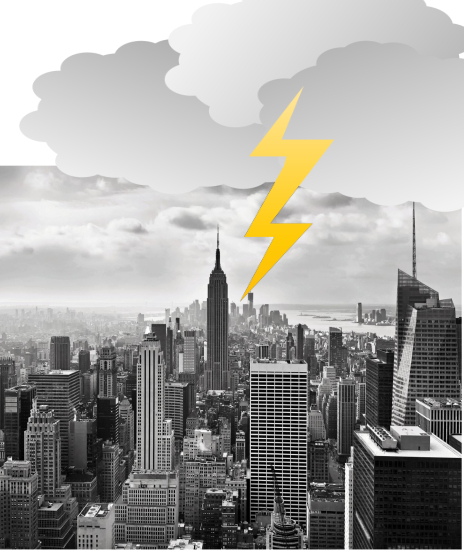
\includegraphics[scale=.45]{graphics/lightning1.jpeg}};  
 \end{tikzpicture}
 
\begin{textblock}{1}(.05,.21)
  \normalsize {Can cityscapes \textbf{influence} weather?}
\end{textblock}
 

\clearpage

%---- slide1b ----------------------------------------------------------


\begin{tikzpicture}[overlay]
  \node[anchor=south west] at (5.5,-5.5) {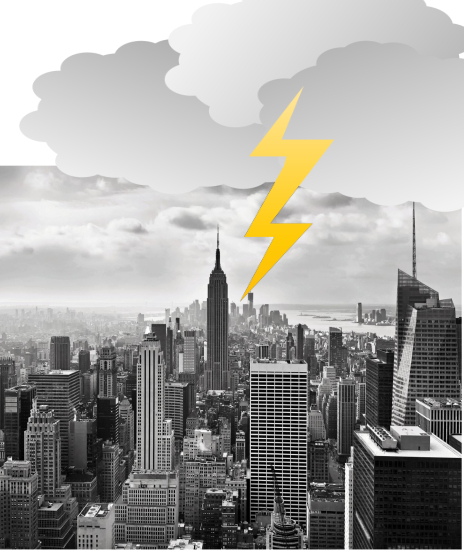
\includegraphics[scale=.45]{graphics/lightning1.jpeg}};  
 \end{tikzpicture}
 
\begin{textblock}{1}(.05,.21)
  \normalsize {Can cityscapes \textbf{influence} weather?}
\end{textblock}
 

\begin{textblock}{1}(.125,.26)
  \normalsize {Can cityscapes \textbf{generate} weather?}
\end{textblock}
 
  
\clearpage


%---- slide1c ----------------------------------------------------------


\begin{tikzpicture}[overlay]
  \node[anchor=south west] at (5.5,-5.5) {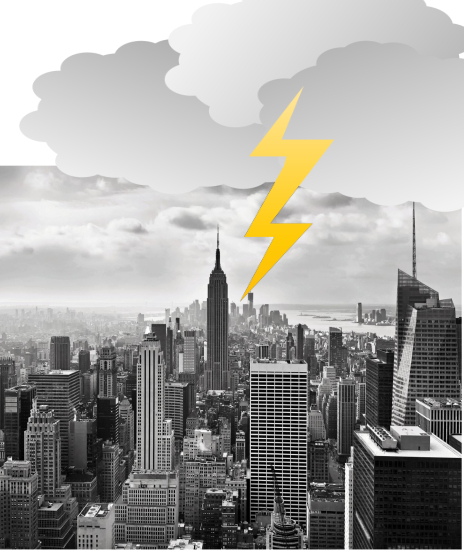
\includegraphics[scale=.45]{graphics/lightning1.jpeg}};  
 \end{tikzpicture}
 
\begin{textblock}{1}(.05,.21)
  \normalsize {Can cityscapes \textbf{influence} weather?}
\end{textblock}
 

\begin{textblock}{1}(.125,.26)
  \normalsize {Can cityscapes \textbf{generate} weather?}
\end{textblock}
 
  
\begin{textblock}{1}(.225,.31)
  \normalsize {Can cityscapes \textbf{cause} thunderstorms?}
\end{textblock}

\clearpage

%---- slide2 ---------------------------------------------------------
\subsubsection{The logic of science: \\
From Reality to models\\
and back again}

\begin{tikzpicture}[overlay]
  \node[anchor=south west] at (6.25,-3.5) {
\includegraphics[scale=.070]{graphics/Jaynes.jpg}};  
 \end{tikzpicture}
 
\begin{textblock}{1}(.045,.40)
  \small {"In virtually all real problems of scientific \\
  inference...the problem facing the scientist \\
  is of the inverse type: Given the data D, \\
  what is the probability that some \\
  hypothesis H is true?"}
\end{textblock}

\begin{textblock}{1}(.2,.60)
  \tiny {--- E.T. Jaynes (2003, p.85)}
\end{textblock}

\clearpage



%---- slide3a ----------------------------------------------------------

\begin{tikzpicture}[overlay]
  \node[anchor=south west] at (1.25,-5.5) {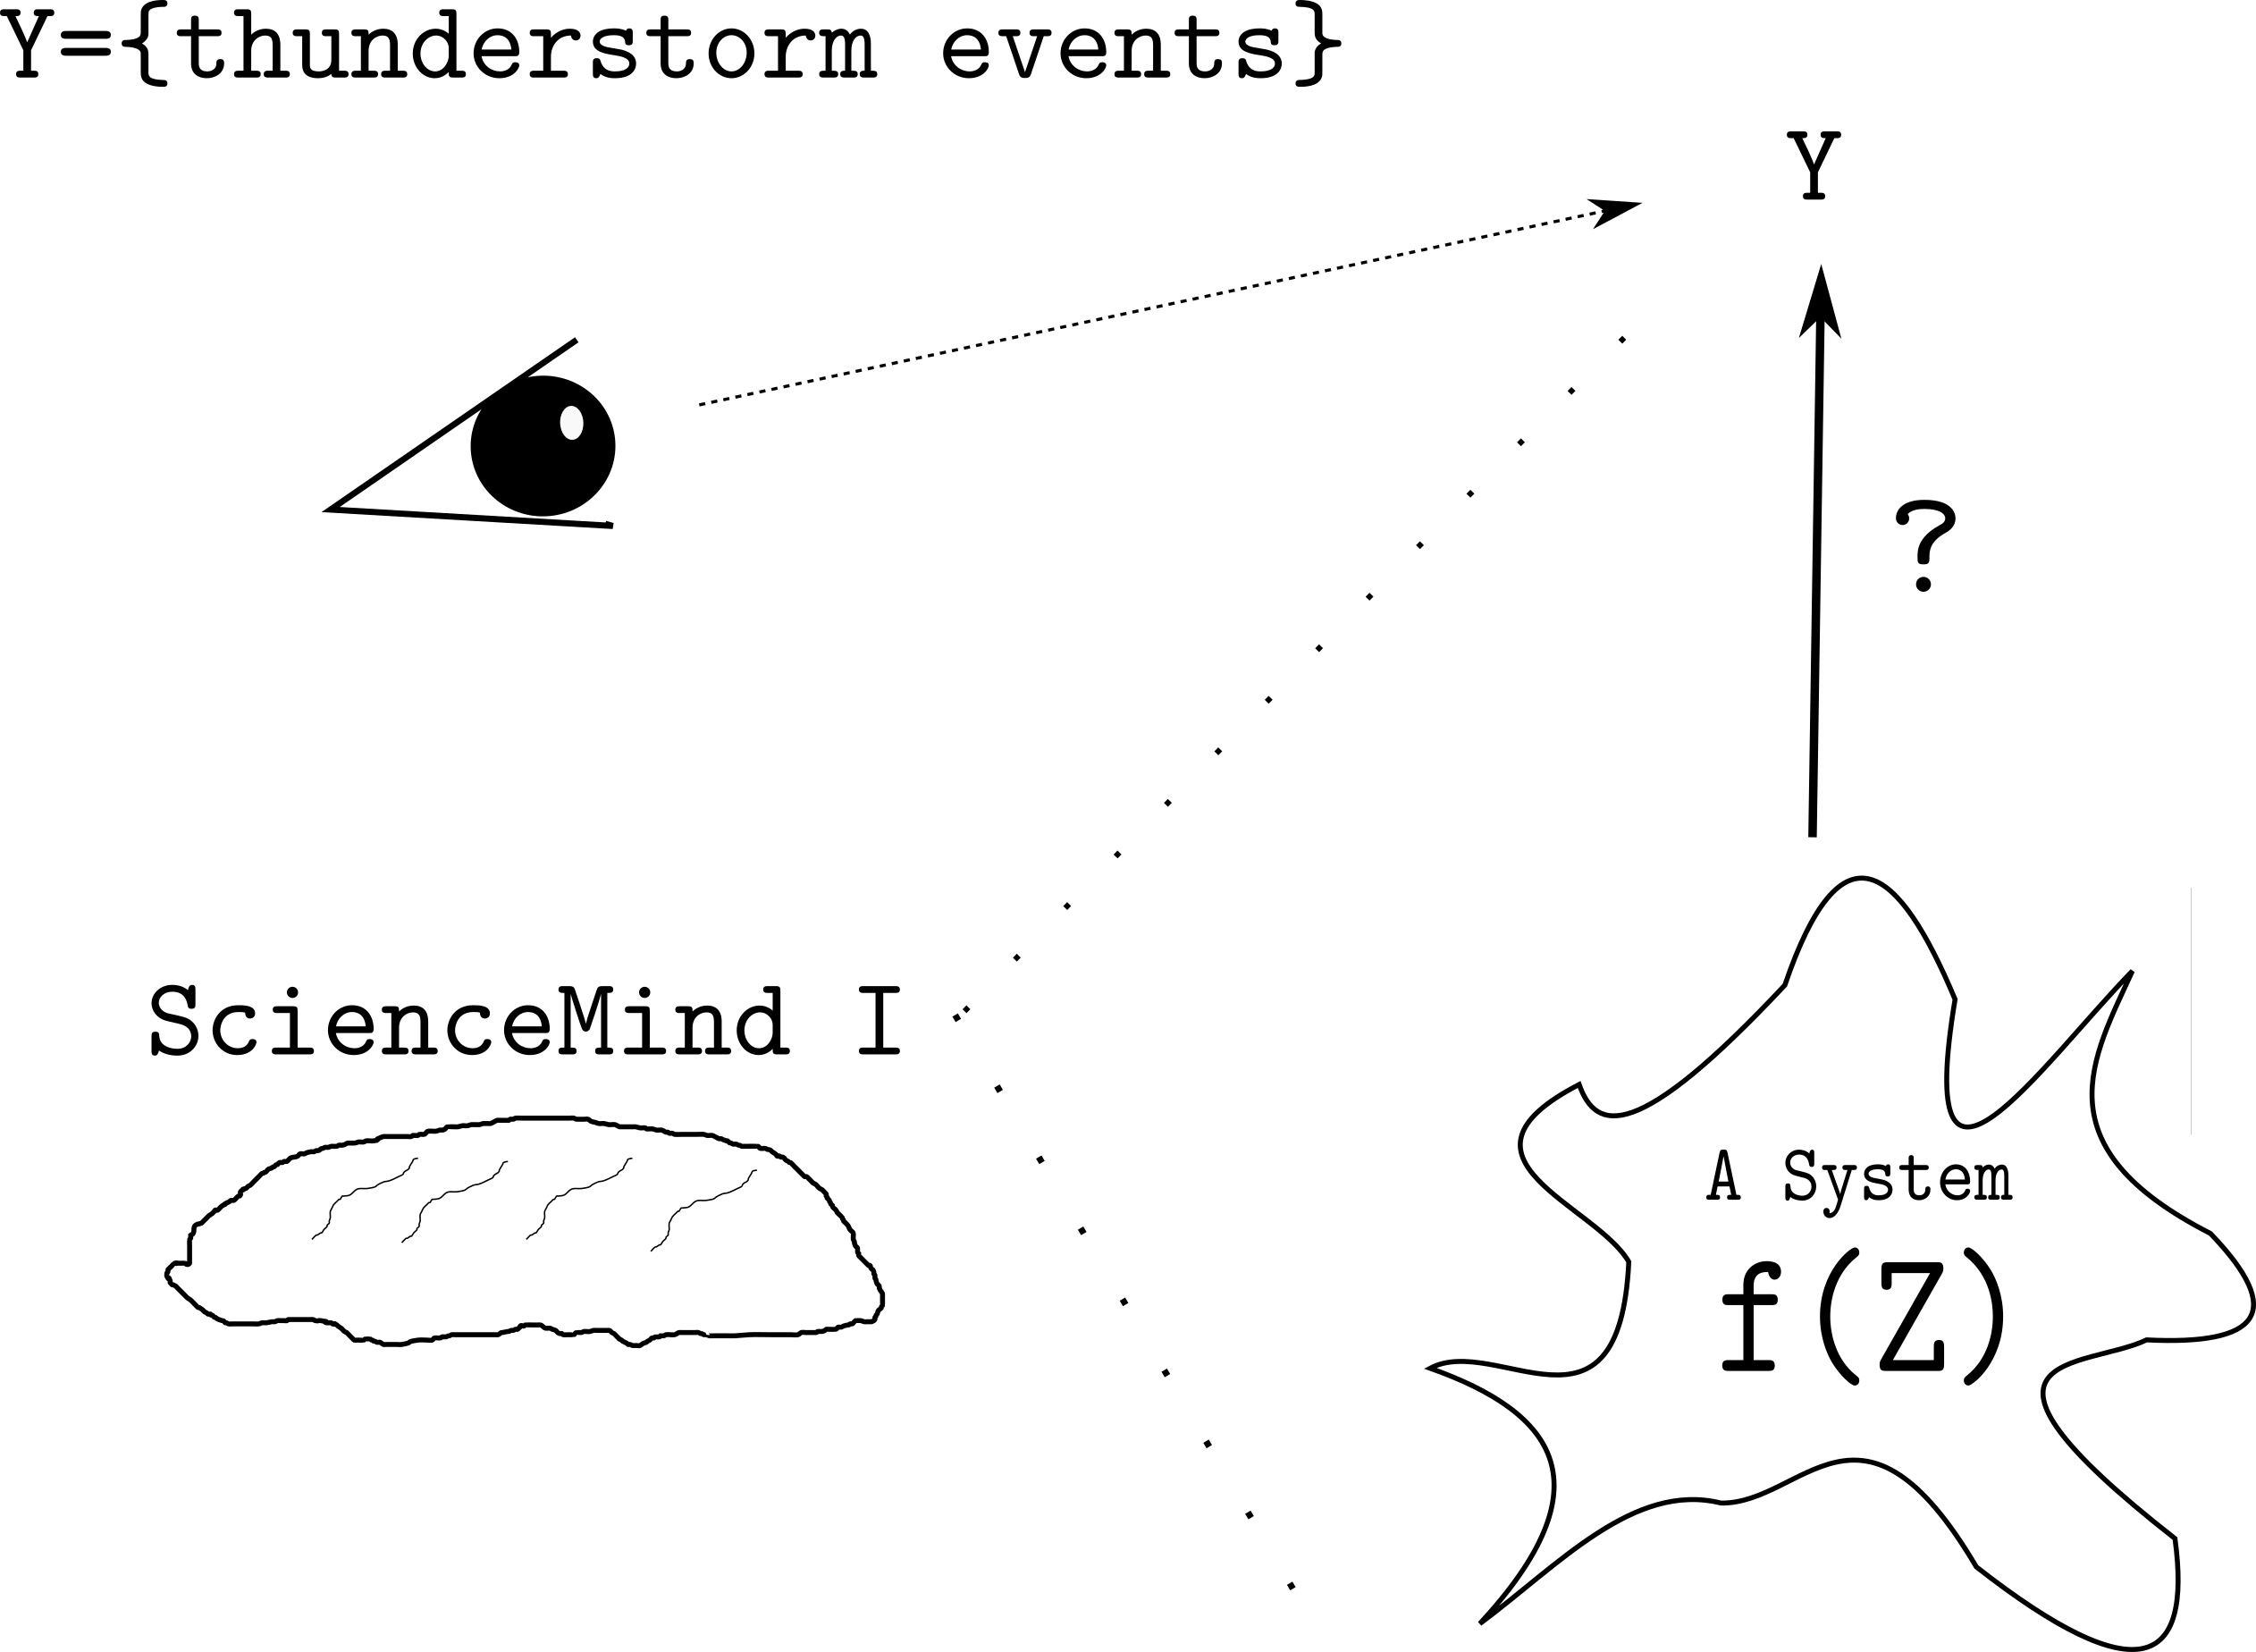
\includegraphics[scale=.75]{graphics/drawing1a}}; 
 \end{tikzpicture}
 
 
\clearpage


%---- slide3b ----------------------------------------------------------


\begin{tikzpicture}[overlay]
  \node[anchor=south west] at (1.75,-5.25) {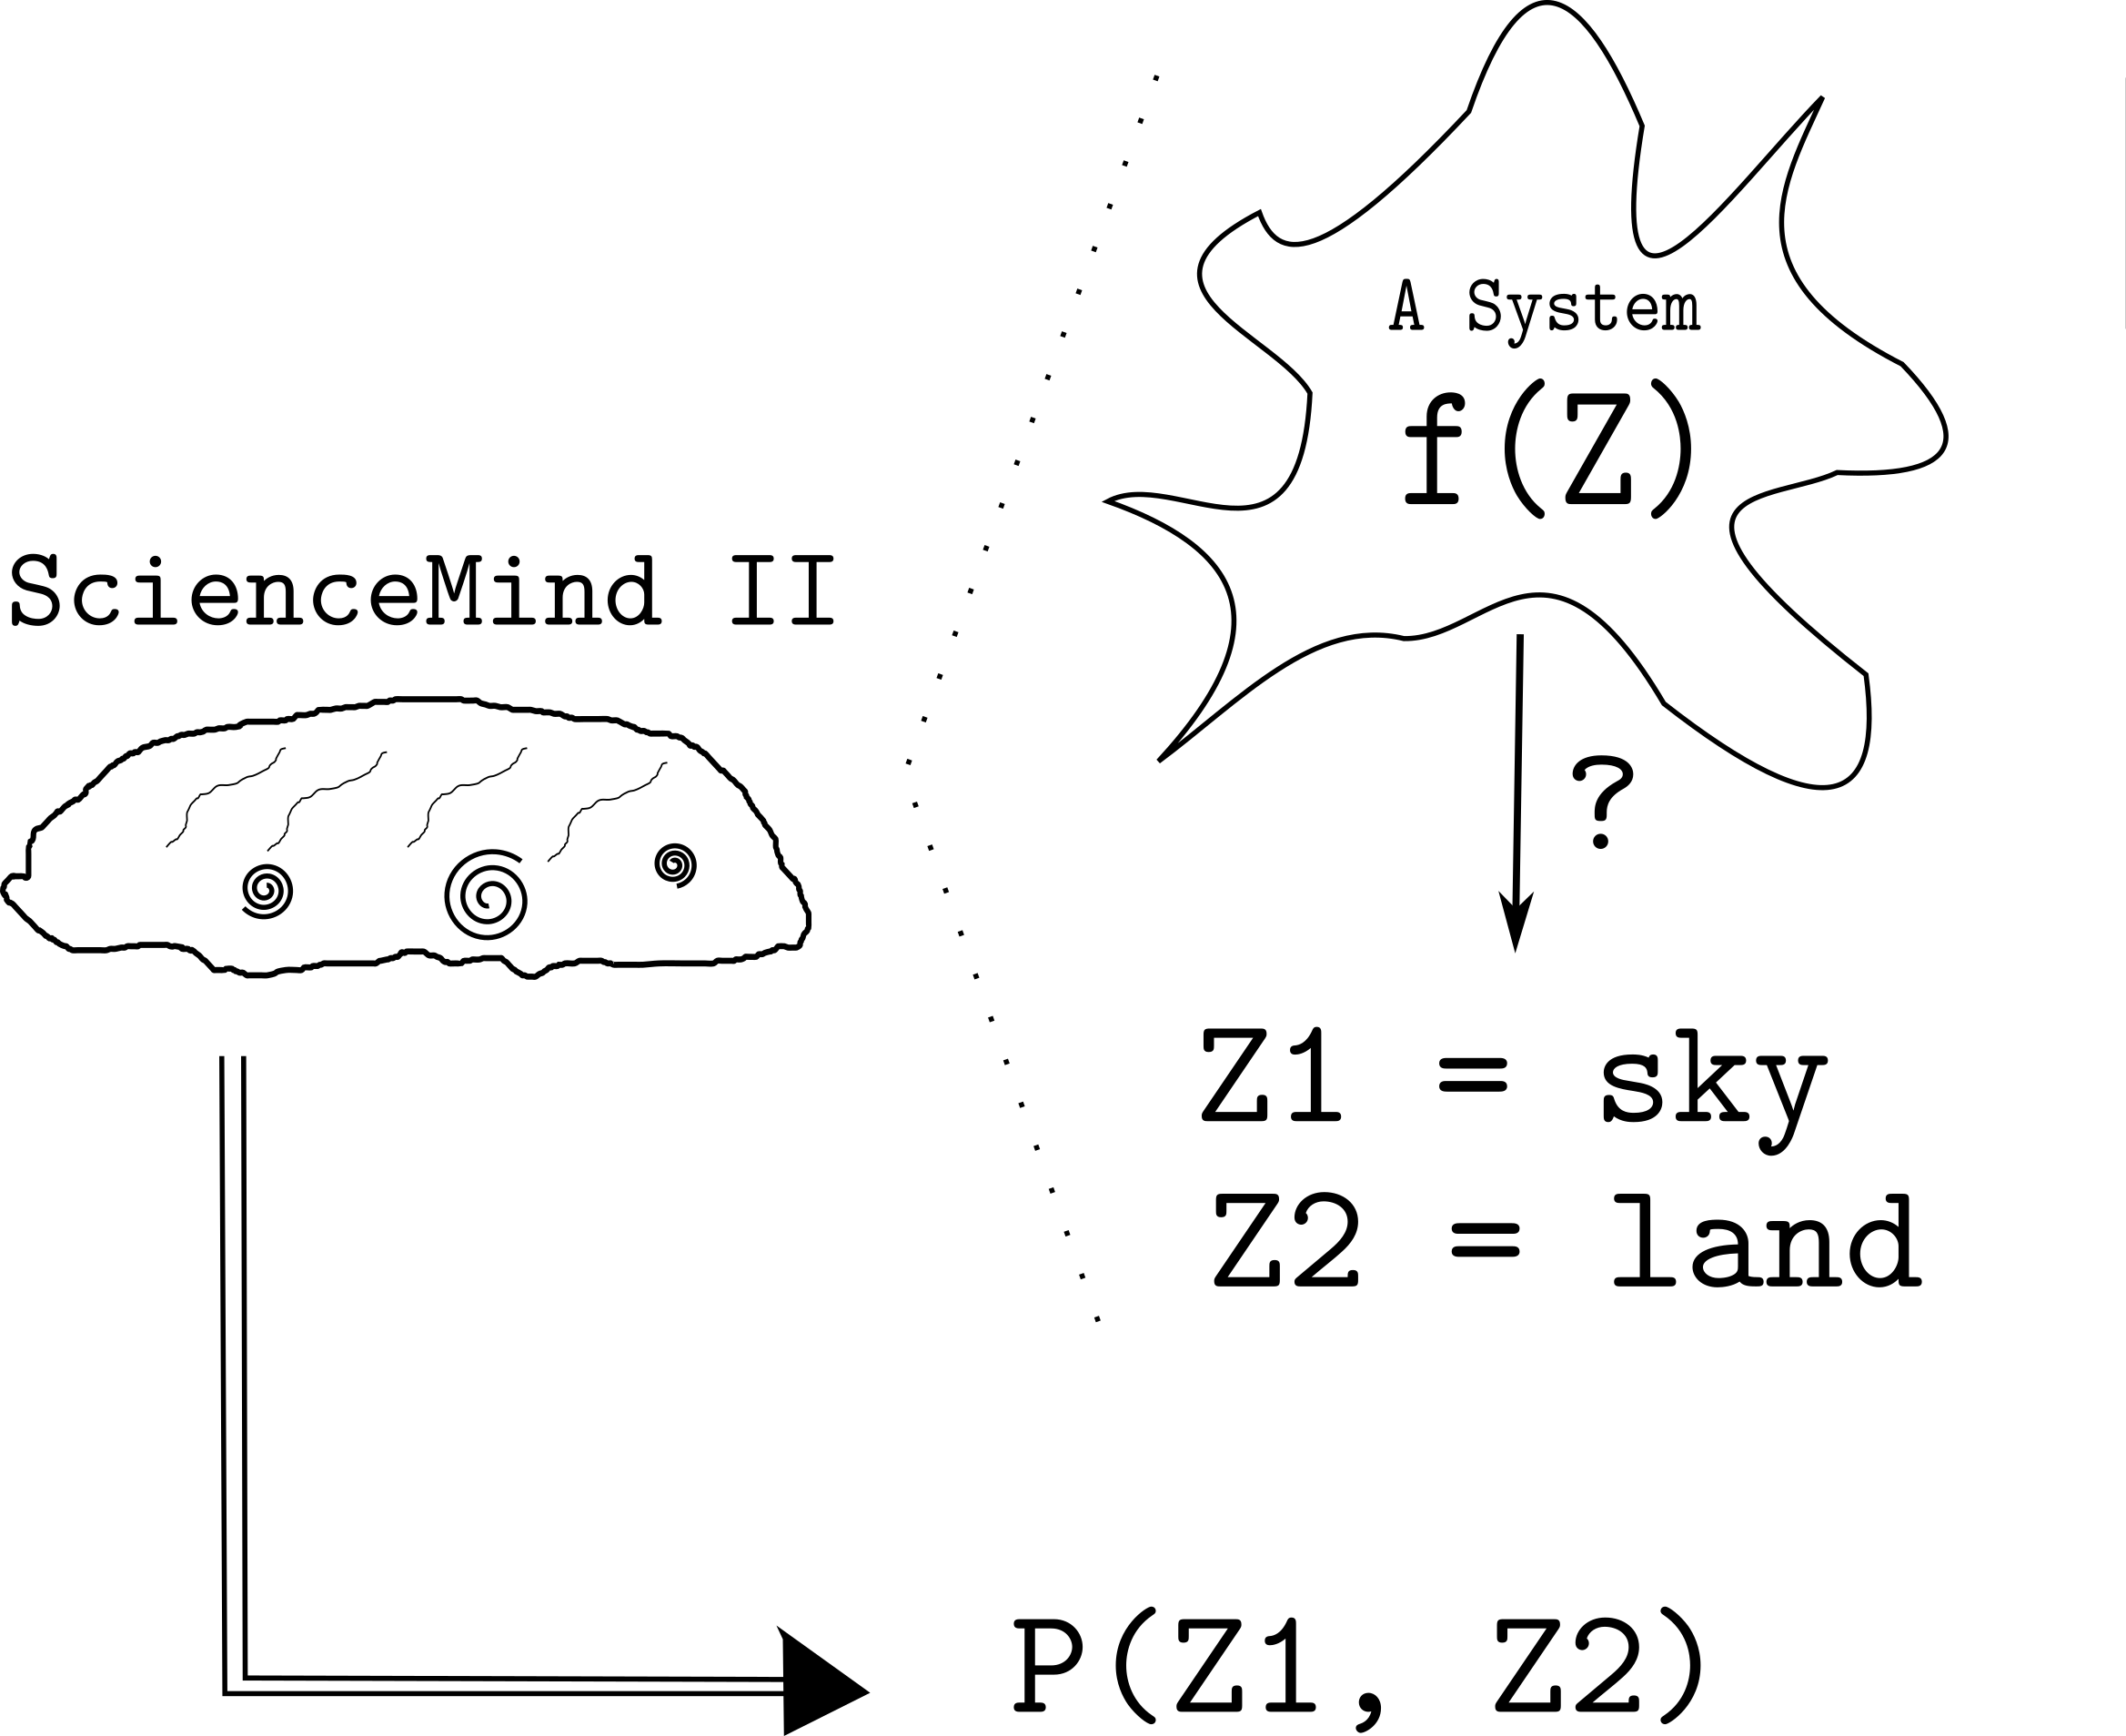
\includegraphics[scale=.70]{graphics/drawing1b}}; 
 \end{tikzpicture}
 
 
\clearpage


%---- slide4 ----------------------------------------------------------


\begin{tikzpicture}[overlay]
  \node[anchor=south west] at (1.75,-5.25) {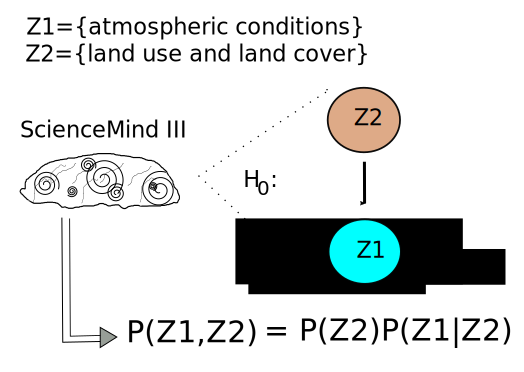
\includegraphics[scale=.70]{graphics/drawing1c}}; 
 \end{tikzpicture}
 
 
\clearpage

%---- slide5 -----------------------------------------------------------

\begin{tikzpicture}[overlay]
  \node[anchor=south west] at (0.5,-1.0) {
\includegraphics[scale=.50]{graphics/Ashley1.jpeg}};
  \node[anchor=south west] at (0.5,-4.0) {
\includegraphics[scale=.50]{graphics/Stallins1.jpeg}};
 \end{tikzpicture}
 
 
 \begin{textblock}{1}(.5,.275)
  \small {... "substantive evidence of urban effects \\ 
  on thunderstorm frequency and severity" ...}
\end{textblock}

 \begin{textblock}{1}(.5,.55)
  \small {"Urban lightning research is still in the \\ 
  descriptive, pattern-identifying stage, \\
  with some inroads into mechanism."}
\end{textblock}

 \clearpage

%---- slide6 ----------------------------------------------------------


\begin{tikzpicture}[overlay]
  \node[anchor=south west] at (1.0,-5.5) {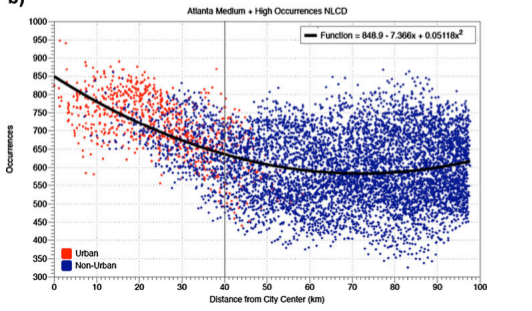
\includegraphics[scale=.75]{graphics/Ashley2.jpeg}}; 
 \end{tikzpicture}
 

\begin{textblock}{1}(.35,.125)
  \footnotesize {$P(Z1, Z2) \ = P(Z2)P(Z1|PZ2)$}
\end{textblock}

\begin{textblock}{1}(.15,.155)
  \footnotesize {$(dBZ = decibels \ radar \ reflectivity \Rightarrow  Z1; NLCD \ code \Rightarrow Z2)$}
\end{textblock}


\begin{textblock}{1}(.10,.20)
  \footnotesize{Occurrences $\geq 40$ dBZ for each 2-km grid cell vs. distance from city center}
\end{textblock}
 
 
\begin{textblock}{1}(.75,.72)
  \tiny {Ashley,Bentley,Stallins (2012)}
\end{textblock}
 
\clearpage



%---- extra slide ------------------------------------------------------------
\subsection{Scientific Inference: From reality to models and back again}

\begin{tikzpicture}[overlay]
  \node[anchor=south west] at (0,-2.0) {
\includegraphics[scale=.35]{graphics/drawing2a}}; 
 \end{tikzpicture}
 
 
 \begin{textblock}{1}(0.40,.25)
  \scriptsize {
  \begin{itemize}
  	\item We observe an entity in Nature that we suspect \\
  	generates non-random patterns of information
  	\item Our states of knowledge about the causal relationships \\
  	and processes, $f(\cdot )$, that are operating as well as about \\
  	the inputs,	$Z$, are limited; often severely	
  	\item We assume that some observable outcome, $Y$, is \\
  	\underline{causally} related to the entity as $f(Z) \Longrightarrow \{Y\}$  	
  \end{itemize}
  }
 \end{textblock}
 
 
\clearpage




%---- extra slide ------------------------------------------------------------
\subsection{Scientific inference: From reality to models and back again}

\begin{tikzpicture}[overlay]
  \node[anchor=south west] at (0,-2.0) {
\includegraphics[scale=.35]{graphics/drawing3}}; 
 \end{tikzpicture}
 
 \begin{textblock}{1}(0.40,.25)
  \scriptsize {
  \begin{itemize}
  	\item We assume that some observable and measurable \\
  	attributes (data), $\{X1, X2\}$ are \underline{logically} related \\
  	 to the entity's internal processes as, $\{X1, X2\} | f(Z) $ 
  	\item Lacking full knowledge of the entity's processes, we use \\
  	a probability model and consider $X1, X2, Y$ as random \\
  	variables with a joint probability distribution function
  	\item Lacking complete datasets, we accept sampled datasets
  	\item We make inductive inferences from the sampled datasets \\
  	back to	$f(Z)$ by assuming sampling distributions, \\
  	evaluating our prior knowledge, and using the (weaker) \\
  	syllogisms of plausible reasoning coupled with probability \\
  	theory
  \end{itemize}
  }
 \end{textblock}
 
 \clearpage
 
 
 

%######################################
% END DOC
%######################################
\end{document}
